\documentclass[conference]{IEEEtran}
\IEEEoverridecommandlockouts
\usepackage{fontspec}
\usepackage{amsmath}
\usepackage{unicode-math}
\setmainfont{STIX Two Text}
\setmathfont{STIX Two Math}
\usepackage{cite}
\usepackage{algorithmic}
\usepackage{graphicx}
\usepackage{textcomp}
\usepackage{xcolor}
\usepackage{booktabs,array}
\def\BibTeX{{\rm B\kern-.05em{\sc i\kern-.025em b}\kern-.08em
    T\kern-.1667em\lower.7ex\hbox{E}\kern-.125emX}}


% Number of participants in the current analyses (update when more subjects are added)
\newcommand{\Nsub}{8}

\begin{document}

\title{Supplementary Material for\\ Category and Load Effects in HCP Working Memory and Language Task-fMRI}

\author{\IEEEauthorblockN{1\textsuperscript{st} Sai Veeksha Tavva}
\IEEEauthorblockA{\textit{IIT Hyderabad} \\
Roll No.\ 2024113021}
\and
\IEEEauthorblockN{2\textsuperscript{nd} Sahishnu Pawan Kumar}
\IEEEauthorblockA{\textit{IIIT Hyderabad} \\
Roll No.\ 2024113016}
}

\maketitle

\setcounter{figure}{0}
\renewcommand{\thefigure}{S\arabic{figure}}
\renewcommand{\thetable}{S\arabic{table}}
\begin{figure*}[t]
\centering
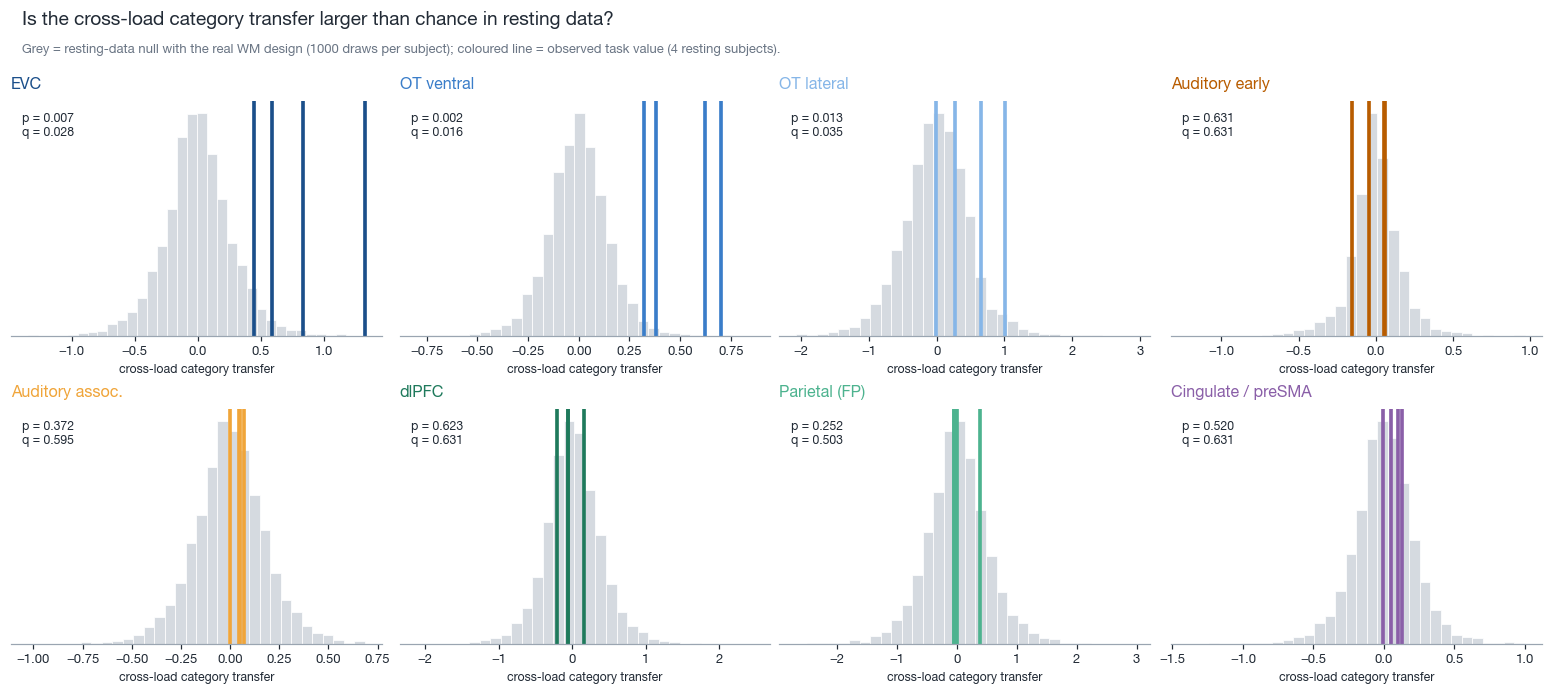
\includegraphics[width=0.97\textwidth]{figures/figS_rest_null.png}
\caption{Group resting-state null for category transfer across load. The grey histogram is what the method gives on resting data with the real task timing. Each coloured line is the task value for one of the four people with resting data. Note: the $p$ and $q$ values printed in the panels come from the first participant only; the group values are given in the text (early visual and OT ventral: $q=0.004$; OT lateral: $q=0.051$; parietal: $q=0.52$).}
\label{figS:restnull}
\end{figure*}
\begin{figure*}[t]
\centering
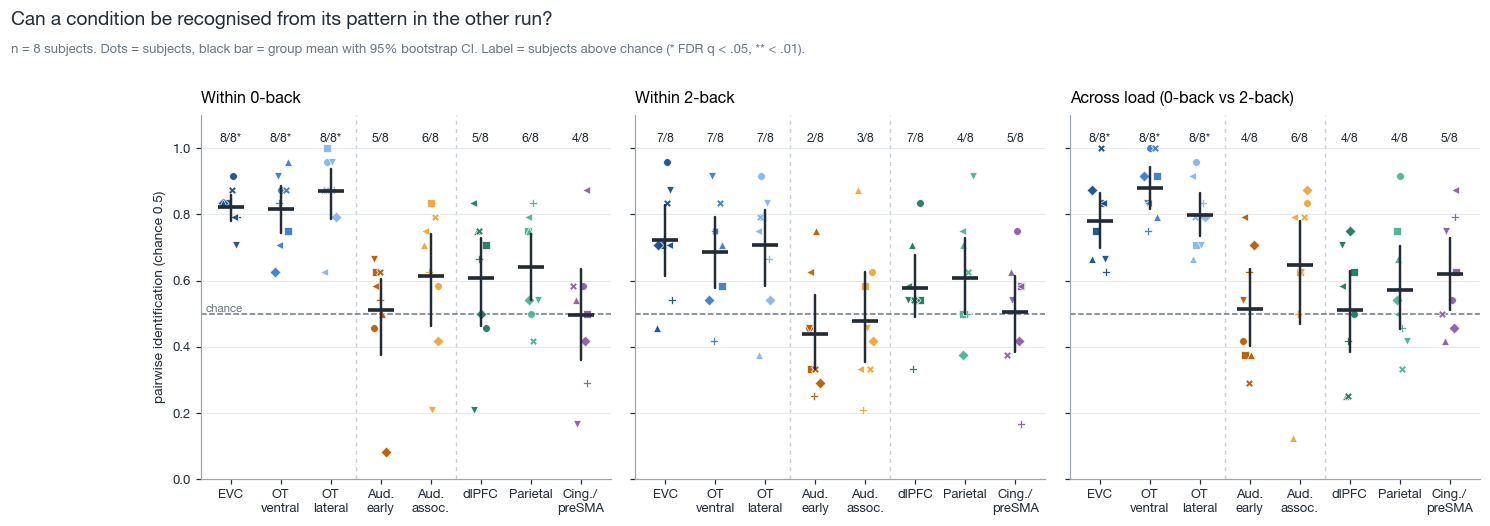
\includegraphics[width=0.97\textwidth]{figures/figS_identification.png}
\caption{Recognising a condition from its pattern in the other run of the same person. Dots are people, the black bar is the group average. The three panels are: within 0-back, within 2-back and across load. The visual regions are reliable in every panel; no other region is.}
\label{figS:ident}
\end{figure*}
\begin{figure*}[t]
\centering
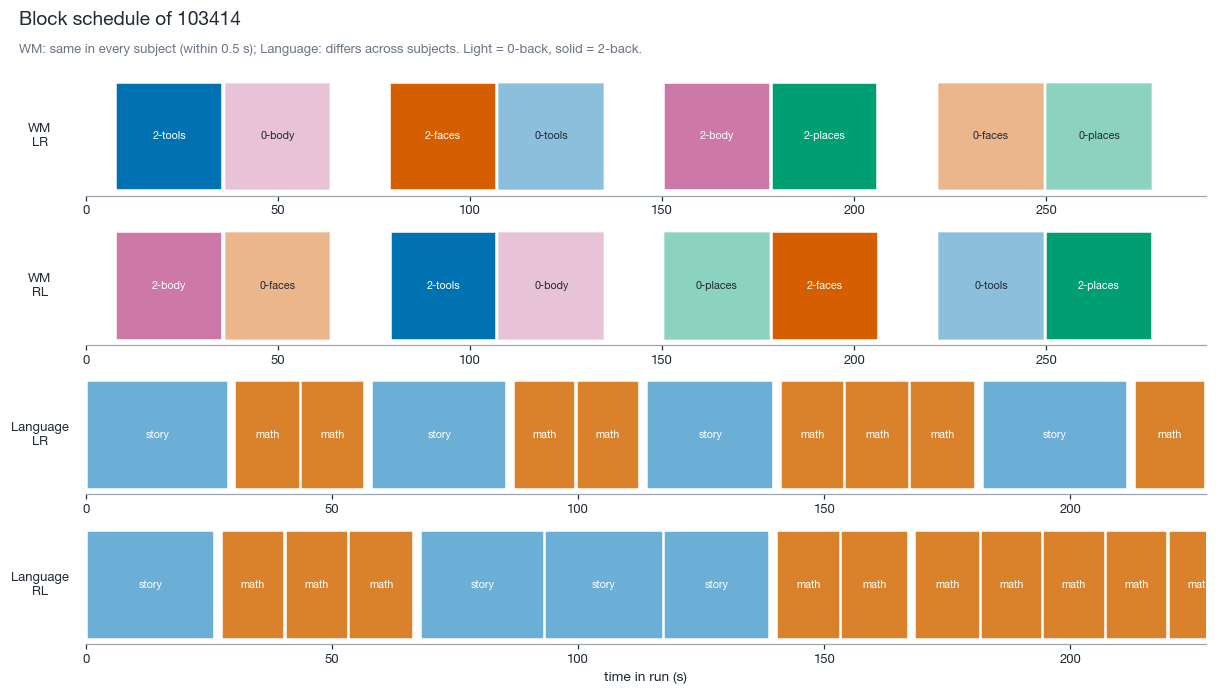
\includegraphics[width=0.97\textwidth]{figures/figS_schedule.png}
\caption{Block schedule of one participant. The working-memory blocks (top) are at the same times in every participant, so the places blocks fall late in both runs. The Language blocks (bottom) differ between participants. Light colours are 0-back and solid colours are 2-back.}
\label{figS:schedule}
\end{figure*}
\begin{figure*}[t]
\centering
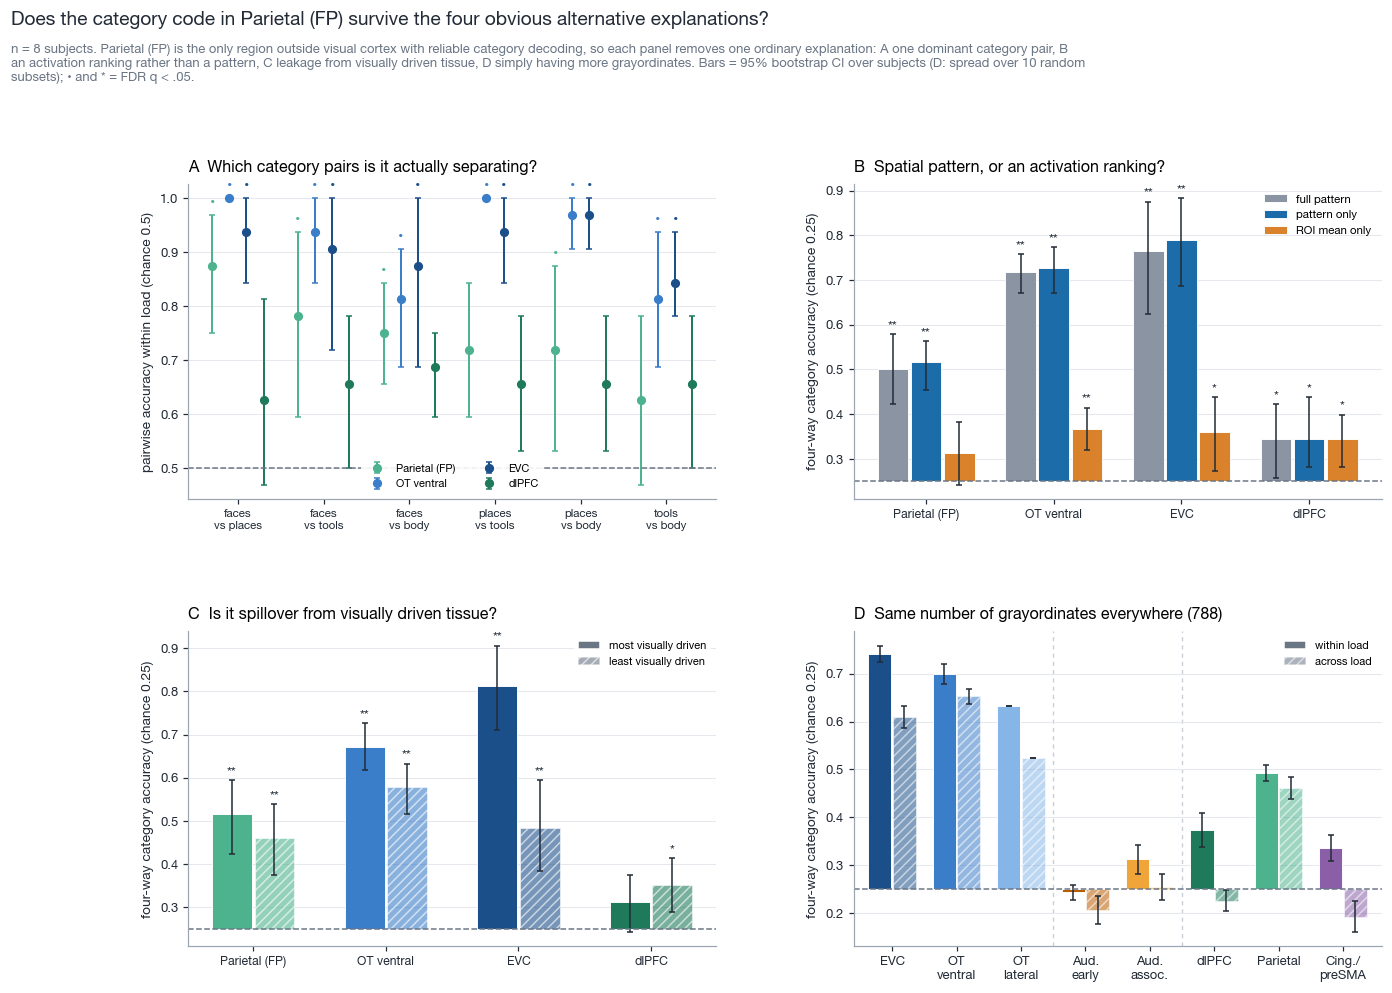
\includegraphics[width=0.97\textwidth]{figures/figS_parietal_checks.png}
\caption{Four checks on the parietal category result. A: which category pairs are separated; B: whether the signal is a spatial pattern or only average activity; C: whether it could leak from the most visually driven locations; D: results with the same number of locations in every region.}
\label{figS:parietal}
\end{figure*}
\begin{figure*}[t]
\centering
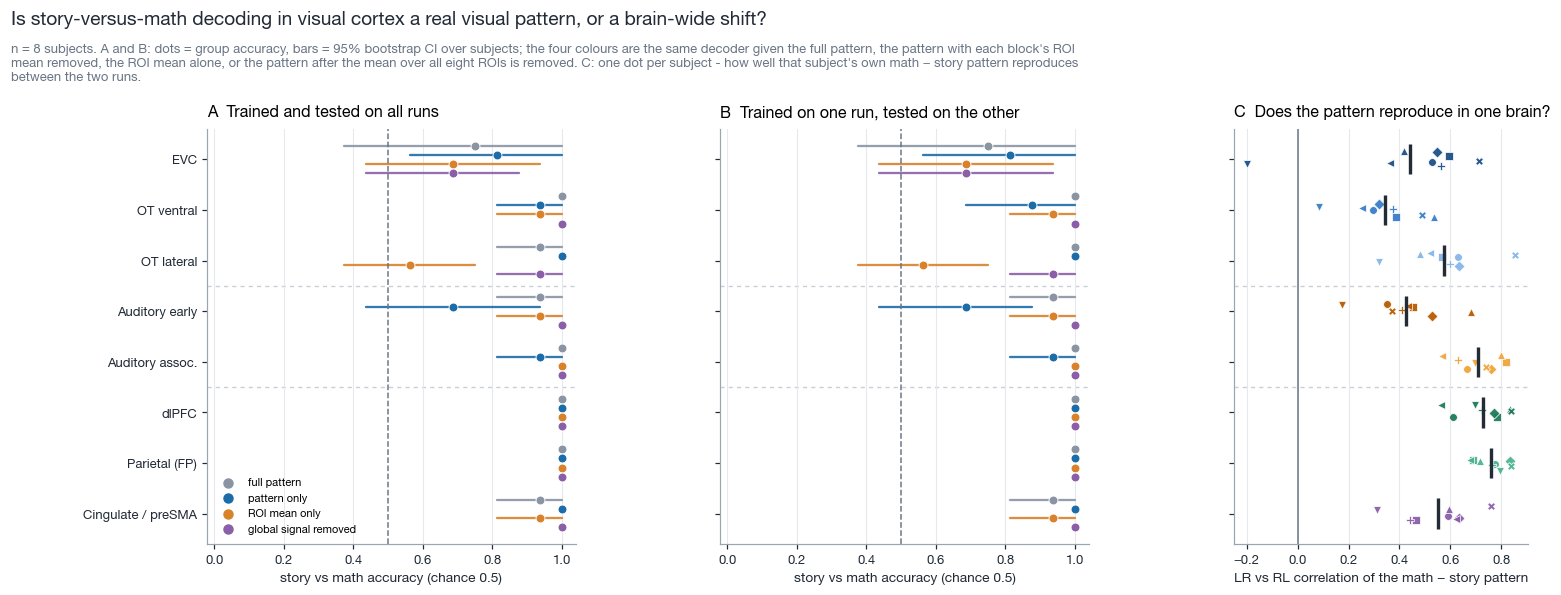
\includegraphics[width=0.97\textwidth]{figures/figS_story_math_visual.png}
\caption{Is Story versus Math in visual cortex a real visual pattern or a brain-wide shift? A and B: accuracy with the full pattern, with each block's average removed, with the average alone, and after removing the average over all regions. C: how well each person's own Math-minus-Story pattern repeats between the two runs.}
\label{figS:storymath}
\end{figure*}
\begin{figure*}[t]
\centering
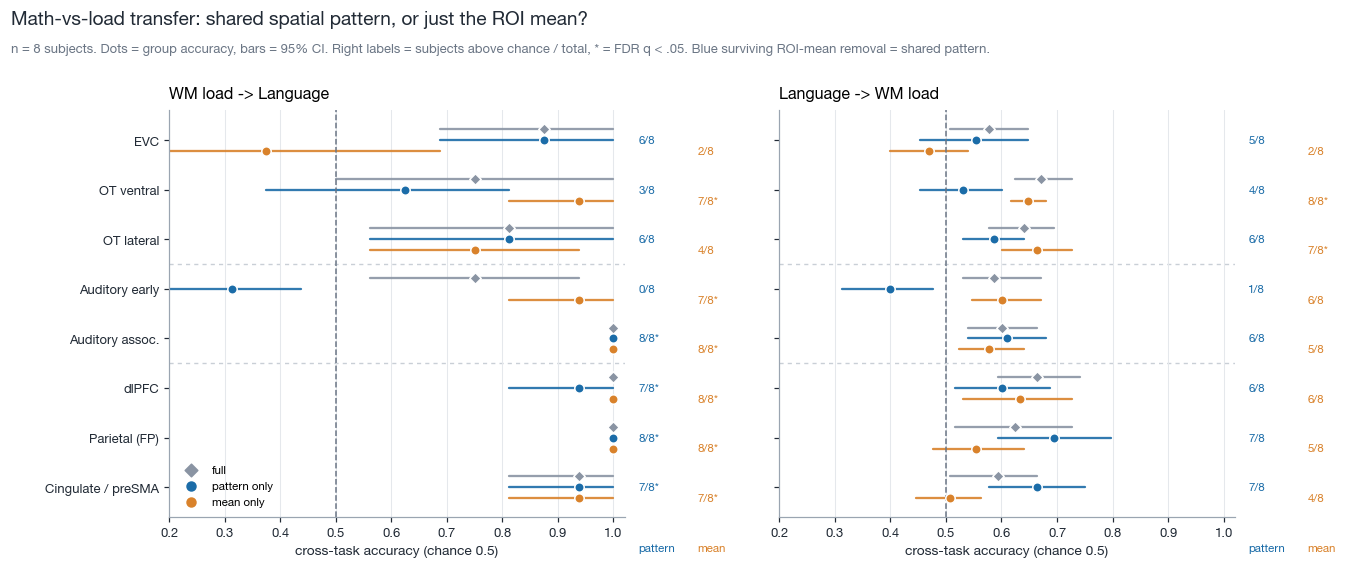
\includegraphics[width=0.97\textwidth]{figures/figS_crosstask_pattern_mean.png}
\caption{Memory-load decoder applied to Math versus Story (left) and the reverse (right), shown for the full pattern, the pattern with the average removed, and the average alone. Blue results that survive removal of the average reflect a shared spatial pattern; orange results reflect average activity.}
\label{figS:crosstask}
\end{figure*}
\begin{figure*}[t]
\centering
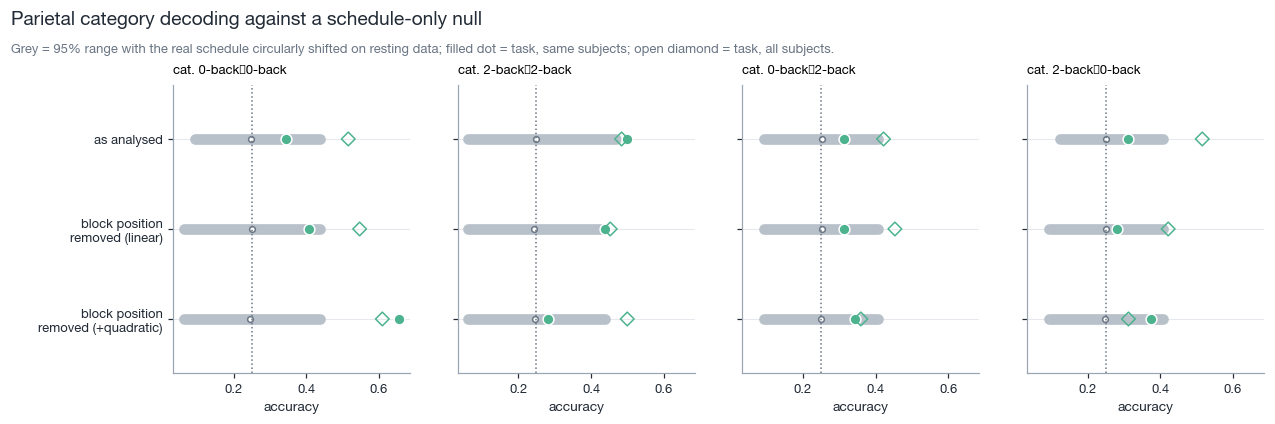
\includegraphics[width=0.97\textwidth]{figures/figS_rest_shift_position.png}
\caption{Parietal category decoding against a schedule-only null. Grey bars are the 95\% range of 1000 draws in which the real task timing was shifted in time and laid over resting data (four people); the small circle is the null mean. The filled dot is task accuracy on the same four people, and the open diamond is task accuracy on all eight. Rows: as analysed, with each block's position in the run removed (linear), and removed (linear plus quadratic). Panel titles read train load $\to$ test load. Across load (panels 3 and 4) the task never leaves the grey bar.}
\label{figS:shift}
\end{figure*}
\begin{table}[t]
\caption{Parietal category decoding, four people, 1000 shifted-schedule draws. Acc.\ is task accuracy on the same four people; $p$ is one-sided against the draws; $q$ is corrected across all regions, analyses and versions.}
\label{tabS:shift}
\centering\small
\begin{tabular}{llcccc}
\toprule
Version & Train$\to$test & Acc. & Null 95\% & $p$ & $q$ \\
\midrule
As analysed & 0$\to$0 & 0.34 & 0.41 & 0.211 & 0.34 \\
 & 2$\to$2 & 0.50 & 0.44 & 0.014 & 0.034 \\
 & 0$\to$2 & 0.31 & 0.38 & 0.273 & 0.42 \\
 & 2$\to$0 & 0.31 & 0.38 & 0.271 & 0.42 \\
Linear & 0$\to$0 & 0.41 & 0.41 & 0.085 & 0.17 \\
 & 2$\to$2 & 0.44 & 0.41 & 0.042 & 0.095 \\
 & 0$\to$2 & 0.31 & 0.41 & 0.297 & 0.44 \\
 & 2$\to$0 & 0.28 & 0.38 & 0.425 & 0.55 \\
Linear + quad. & 0$\to$0 & 0.66 & 0.41 & 0.001 & 0.004 \\
 & 2$\to$2 & 0.28 & 0.41 & 0.420 & 0.55 \\
 & 0$\to$2 & 0.34 & 0.38 & 0.172 & 0.30 \\
 & 2$\to$0 & 0.38 & 0.38 & 0.096 & 0.19 \\
\bottomrule
\end{tabular}
\end{table}

\end{document}
